%!TEX root = main.tex
  \section{\change{Related Works\label{sec:relatedworks}}}
\change{
  % \subsection{Background and Motivation}
  \npar We will now describe past work in visual query systems and existing evaluation methods of visualization systems to provide background and motivation to our work. Then, we will introduce Pirolli and Card's sensemaking model, which serves as a framework for contextualizing our study findings. 
  % Visual query systems enable users to directly search for visualizations matching certain patterns through an intuitive specification interface. Early work in this space focused on interfaces to search for time series with specific patterns.
  \par \stitle{Visual Query Systems: Definition and Brief Survey}
  \npar \emph{Visual query system} (VQS) is a term coined by Ryall et al. and Correll and Gleicher\cite{ryall2005querylines,correll2016semantics} to describe systems that enable analysts to directly search for time-series visualizations matching certain patterns through an intuitive specification interface. Examples of such systems include TimeSearcher~\cite{Hochheiser2001,Hochheiser2004}, where the query specification mechanism is a rectangular box, with the tool filtering out all of the time series that does not pass through it, QuerySketch~\cite{wattenberg2001sketching} and Google Correlate~\cite{mohebbi2011google}, where the query is sketched as a pattern on canvas, with the tool filtering out all of the time series that have a different shape. Subsequent work recognized the ambiguity in sketching by studying how humans rank the similarity in patterns~\cite{Eichmann2015,correll2016semantics,Mannino2018} and improving the expressiveness of sketched queries through finer-grained specification interfaces and pattern-matching algorithms~\cite{ryall2005querylines,Holz2009}. In our work, we built on an existing VQS, \zv~\cite{Siddiqui2017,Siddiqui2017VLDB}, that allowed users to sketch a pattern or drag-and-drop an existing visualization as a query, with the system returning visualizations that had the closest Euclidean distance to the queried pattern. We chose to build on top of \zv, since it was open-source, extensible, and included features beyond pattern and match specification typically found in existing systems, as compared in Table~\ref{table:relatedwork}.% and described in Section~\ref{sec:sensemaking}. 
  %performed crowdsourced perceptual studies to understand how humans rank similarity in patterns subjectively
  % , including the use of soft constraints~\cite{ryall2005querylines} and implicit relaxed selection techniques~\cite{Holz2009}.
  % In addition to this ongoing work, recent work have also performed crowdsourced perceptual studies to understand how humans rank similarity in patterns subjectively~\cite{Eichmann2015,correll2016semantics,Mannino2018}.
  \begin{table}[h!]
    \vspace*{-10pt}
     \centering
     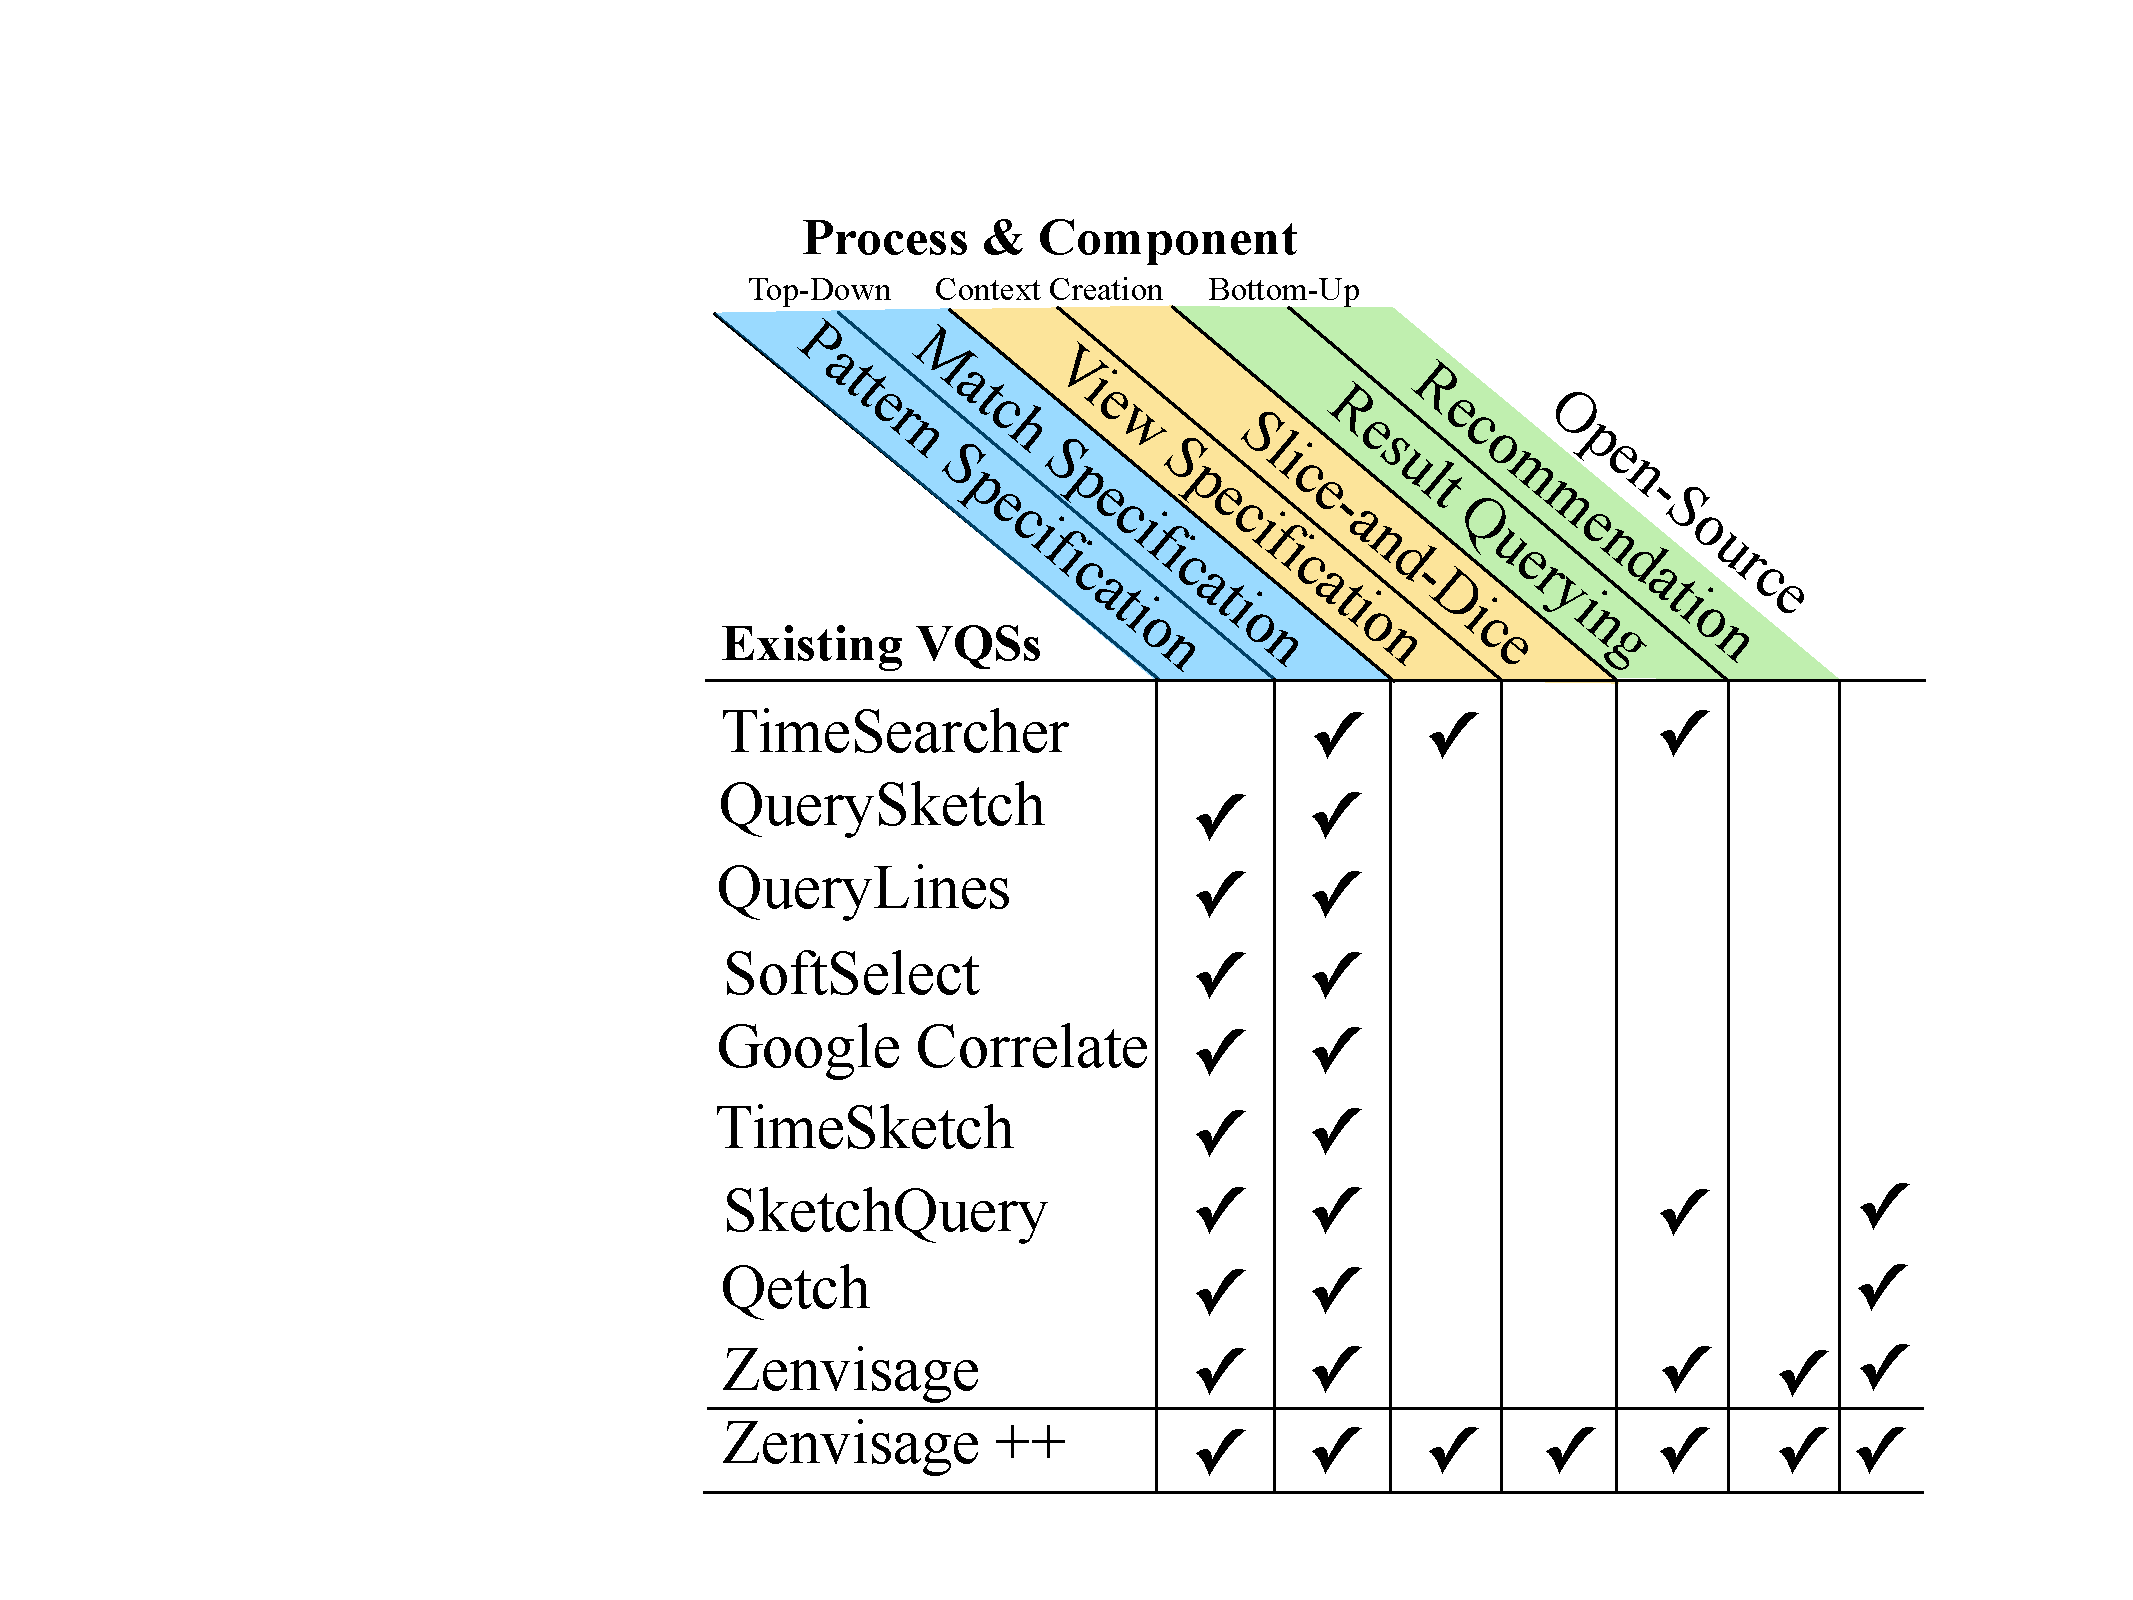
\includegraphics[width=0.8\linewidth]{figures/related_works_table.pdf}
     \caption{Table summarizing whether key functional components (columns) are covered by past systems (row), indicated by checked cells. Column header colors blue, orange, green represents three sensemaking process (top-down querying, search with context, and bottom-up querying) described in Section~\ref{sec:pd_findings}. The heavily-used, practical features in our study for context-creation and bottom-up inquiry is largely missing from prior VQSs.}
     \label{table:relatedwork}
     \vspace*{-15pt}
  \end{table}
  \par \stitle{Design and Evaluation Methodologies for Visualization Systems}
  \npar Visualization systems are typically evaluated via in-lab usability studies or controlled studies against existing visualization baselines~\cite{Plaisant2004,North2006,Yi2008}. However, successful lab-tested systems do not always translate to community acceptance and adoption. For instance, while decades of work have shown VQSs to be effective in controlled lab studies, they have not gained widespread adoption. \cut{Unlike our work, past VQSs have never been designed and evaluated in-situ on multiple real-world use cases. Even when use cases were involved~\cite{Hochheiser2004,correll2016semantics}, the inclusion of these case studies served as a post-hoc demonstrative case study that had little influence on the major design decisions of the system.} In the context of Munzner's nested model~\cite{munzner2009nested}, this gap between research and adoption stems from the common ``downstream threat'' of jumping prematurely into the deep levels of \textit{encoding, interaction, or algorithm design}, before a proper \textit{domain problem characterization} and \textit{data/operation abstraction design} is performed. Our work aims to fill this crucial gap in the existing literature.
  \par The unrealistic nature of controlled studies have prompted the visualization research community to propose a more participant-centered, ethnographic approach to understand how analysts perform visual data analysis and reasoning~\cite{Plaisant2004,lam2012empirical,shneiderman2006strategies,munzner2009nested,Sedlmair2012}. For example, multi-dimensional, in-depth, long-term case studies (MILCs) advocate the use of interviews, surveys, logging and other empirical artifacts to create a holistic understanding of how a visualization system is used in its intended environment \cite{shneiderman2006strategies}. 
  \par In this work, we performed design studies~\cite{lam2012empirical,shneiderman2006strategies,Sedlmair2012} with three different subject areas for \textit{domain problem characterization} by adopting \emph{participatory design} practices~\cite{Gould1983,Muller1993} to engage potential stakeholders in designing a VQS that they may eventually use in their analytical workflow. Participatory design is well-established in the CHI and CSCW community and has been successfully applied to develop systems for visual analytics~\cite{Aragon2008,Chuang2012}, tangible museum experiences~\cite{Ciolfi2016}, and scientific collaborations~\cite{Poon2008,Chen2016} in the past. Past research on participatory design has found that the use of functional prototypes is a common and effective way of engaging with participants and providing a starting point for participatory design~\cite{Ciolfi2016}. Similarly, we provide a functional prototype at the beginning of the participatory design sessions was to showcase capabilities of VQSs. \cut{Since our participants were not aware of the existence of VQSs, let alone using them in their workflows, they would not have been able to imagine use cases for VQS without a starting point.} Likewise, the use of ``\textit{simulated future work situation}'' is also a common practice in cooperative prototyping when the real use of the prototype is not feasible~\cite{Grnbak1991}. To better understand how VQSs can be used in-situ participant's existing workflow, we regularly gathered feedback from participants and collaboratively envisioned potential designs based on previews of preliminary versions of our protoype \zvpp. Finally, we validated our abstraction design with grounded evaluation~\cite{Plaisant2004,Isenberg2008}, where we invited participants to bring in their own datasets and research problems that they have a vested interest in to test our final deployed system.
  %Sedlmair et al. \cite{Sedlmair2012} highlights the benefits and pitfalls of design studies in visualization research. They advocate that design study methodology is suitable for use cases in which the data is available for prototyping, but the task is only partially known and the information is partially in the user's head. In that regard, our scientific use cases with VQS is well-suited for a design study methodology, as we learn about the scientist's data and analysis requirements and design interactions that helps users translate their ``in-the-head'' specifications into actionable visual queries. 
  %\par While these systems have been effective in controlled lab studies, they have never been designed and evaluated in-situ on multiple real-world use cases. Even when use cases were involved~\cite{Hochheiser2004,correll2016semantics}, the inclusion of these \change{case studies served as a post-hoc demonstrative case study that had} little influence on the major design decisions of the system. 
 %\change{Next, we will outline these two phases of our study, deferring details of the study procedures and protocols to the technical report.}%Next, we will describe these two phases of our study in more detail.
  \par \stitle{Sensemaking Models for Visual Analytics}
  \npar Based on our participatory design findings, we contribute to the \textit{data/operation abstraction design} of VQSs by developing a taxonomy for understanding how analysts make use of VQSs to accomplish their analytical tasks. To develop a sensemaking model for VQS, we draw from Pirolli and Card's seminal paper on information foraging~\cite{Pirolli} based on cognitive task analysis. The sensemaking framework was designed to capture how expert analysts perform intelligence analysis in the act of iteratively searching and re-representing the gathered evidence into a conceptual model (\emph{schema}). Based on this framework, the sensemaking process can organized into 1) a foraging loop that searches for information for further organization into a schema and 2) a sensemaking loop for constructing a schema that best aligns with the insights obtained from the analysis. Overall, the model distinguishes between information processing tasks that are \textit{top-down} (from theory to data) and \textit{bottom-up} (from data to theory). We were inspired by this model for expert intelligence analysis as it bears bearing semblance to our work for studying how domain experts perform visual analysis using VQSs.
  \par Many work in visual analytics applied the sensemaking framework to motivate tool design decisions, such as in exploratory visual browsing of large datasets~\cite{Battle2016} and web-search and browsing~\cite{Olston2003}. In addition, the sensemaking framework have also been used for understanding and modelling user behavior in visual analytics, including how analysts gain insights from visualizations~\cite{Yi2008}, how bias can be introduced and accumluated across sensemaking cycles~\cite{Wall2017}, and how analysts transition between natural-language generated data facts and visualizations~\cite{Srinivasan2019}.
% Our VQS sensemaking model is inspired by Pirolli and Card's information foraging framework~\cite{Pirolli}, which distinguishes between information processing tasks that are \textit{top-down} (from theory to data) and \textit{bottom-up} (from data to theory).





   
  
% We analyze our participatory deisng findings through the lens of
  
 } 
  